% gc-05-TrigDiff.tex

\documentclass[xcolor=dvipsnames]{beamer}

\usepackage{cancel}
\renewcommand{\CancelColor}{\color{red}}
\usepackage{graphicx}
\usepackage{wrapfig}
\usepackage{colortbl}
\definecolor{myblue}{rgb}{0.8,0.85,1}

\mode<presentation>
{
  \usetheme{Warsaw}
  \setbeamercovered{transparent}
}
% \usecolortheme[named=OliveGreen]{structure}
\setbeamertemplate{navigation symbols}{} 
\setbeamertemplate{blocks}[rounded][shadow=true] 

\newif\ifBCITCourse
\BCITCoursetrue
% \BCITCoursefalse
\newif\ifWhichCourse
\WhichCoursetrue
\WhichCoursefalse
\ifBCITCourse
\ifWhichCourse
\newcommand{\CourseName}{Statistics for Food Technology}
\newcommand{\CourseNumber}{MATH 1441}
\newcommand{\CourseInst}{BCIT}
\else
\newcommand{\CourseName}{Calculus for Geomatics}
\newcommand{\CourseNumber}{MATH 1511}
\newcommand{\CourseInst}{BCIT}
\fi
\else
\newcommand{\CourseName}{Philosophy and Literature}
\newcommand{\CourseNumber}{PHIL 375}
\newcommand{\CourseInst}{UBC}
\fi

\title{Differentiating Trigonometric Functions}
\subtitle{{\CourseNumber}, BCIT}

\author{\CourseName}

\date{January 20, 2017}

% \begin{figure}[h]
% 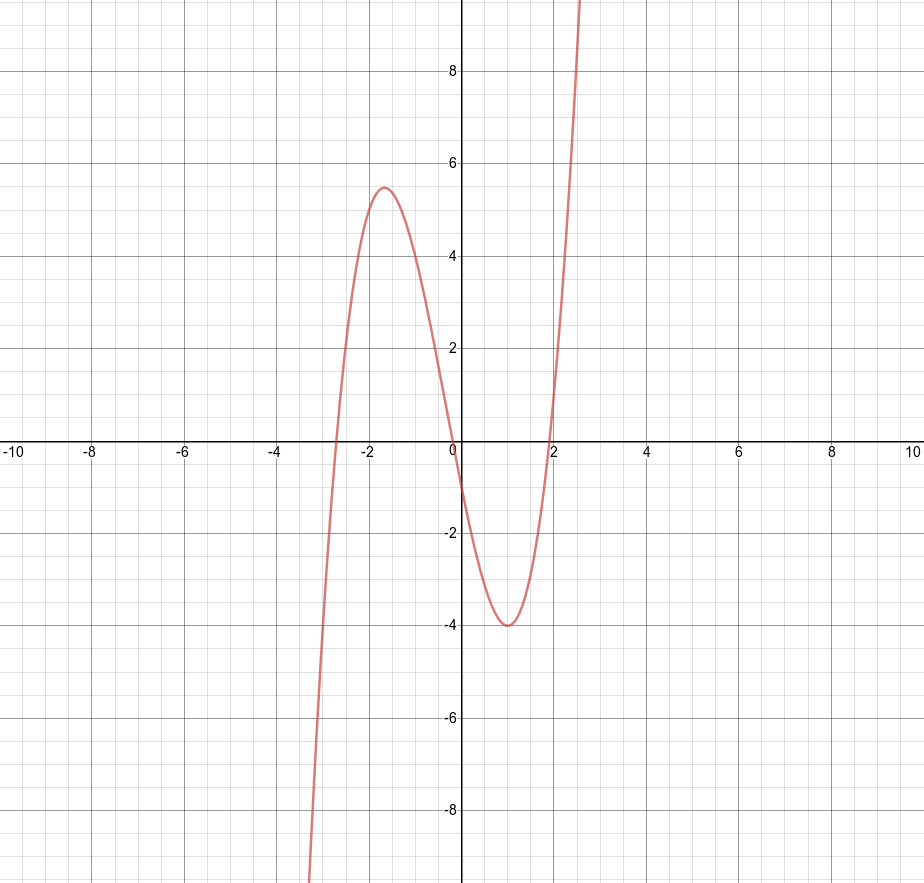
\includegraphics[scale=.3]{./diagrams/extrema1.png}
% \end{figure}

\begin{document}

\begin{frame}
  \titlepage
\end{frame}

\begin{frame}
  \frametitle{The Derivative of Sine}
The derivative of $f(\vartheta)=\sin\vartheta$ is 
\begin{equation}
  \label{eq:eishooro}
  f'(\vartheta)=\cos\vartheta
\end{equation}
For a proof, see James Stewart, \emph{Single Variable Calculus}, Sixth
Edition, page 190f.

\emph{Exercise:} Differentiate $f(x)=x^{2}\sin{}x$.
\end{frame}

\begin{frame}
  \frametitle{The Derivative of Cosine}
The derivative of $f(\vartheta)=\cos\vartheta$ is 
\begin{equation}
  \label{eq:ahfiefev}
  f'(\vartheta)=-\sin\vartheta
\end{equation}
The proof is analogous to the proof for $\sin{}\vartheta$.

\emph{Exercise:} Differentiate 
\begin{equation}
  \label{eq:afeizeix}
  f(t)=\frac{1+\sin{}t}{t+\cos{}t}
\end{equation}
\end{frame}

\begin{frame}
  \frametitle{The Derivative of Tangent}
The derivative of $f(\vartheta)=\tan\vartheta$ is 
\begin{equation}
  \label{eq:uulohjeo}
  f'(\vartheta)=\sec^{2}\vartheta
\end{equation}
Use the quotient rule to prove this. Remember that 
\begin{equation}
  \label{eq:shooceid}
  \sec\vartheta=\frac{1}{\cos\vartheta}
\end{equation}
\end{frame}

\begin{frame}
  \frametitle{Derivatives of Trigonometric Functions}
\begin{figure}[h]
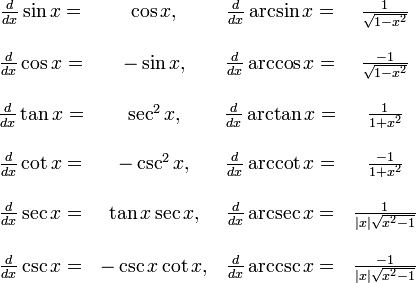
\includegraphics[scale=.6]{./diagrams/trigdiff.png}
\end{figure}
\end{frame}

\begin{frame}
  \frametitle{Exercises}
Differentiate the following functions:
\begin{equation}
  \label{eq:hupuxahz}
  f(x)=3x^{2}-2\cos{}x
\end{equation}
\begin{equation}
  \label{eq:vithooke}
  f(x)=\sqrt{x}\sin{}x
\end{equation}
\begin{equation}
  \label{eq:chaequin}
  f(x)=2\csc{}x+5\cos{}x
\end{equation}
\begin{equation}
  \label{eq:hohxenoo}
  g(t)=4\sec{}t+\tan{}t
\end{equation}
\begin{equation}
  \label{eq:tohsohgh}
  v(w)=\frac{\sin{}w}{w^{2}}
\end{equation}
\begin{equation}
  \label{eq:zichoope}
  f(x)=\csc{}x(x+\cot{}x)
\end{equation}
Find the equation of the tangent line at $(\pi/3,2)$ for
\begin{equation}
  \label{eq:hoirohfo}
  y=\sec{}x
\end{equation}
\end{frame}

\begin{frame}
  \frametitle{End of Lesson}
Next Lesson: Chain Rule
\end{frame}

\end{document}
